\documentclass[a4paper,11pt,twoside,openright]{book}							% COMANDI INIZIALI
\usepackage[italian]{babel}								% sillabazione italiana
\usepackage[utf8]{inputenc}								% Per le lettere accentate IN UNIX E IN WINDOWS
\usepackage{ragged2e}					 				% giustifica
\usepackage{amsmath}									% Per allineare le equazioni
\usepackage{amssymb}									% Per le lettere dell'indicatrice (mathbb)


\usepackage[sc]{mathpazo}
%Options: Sonny, Lenny, Glenn, Conny, Rejne, Bjarne, Bjornstrup
\usepackage[Sonny]{fncychap}
\usepackage{fancyhdr}
\pagestyle{fancy}
\fancyhead{} % cancella tutti i campi
\fancyfoot{}
\fancyhead[RE,LO]{\slshape \leftmark}
\fancyhead[LE,RO]{\thepage}
\renewcommand{\headrulewidth}{0.4pt}
%\renewcommand{\footrulewidth}{0.4pt}
\renewcommand{\chaptermark}[1]{%
\markboth{\thechapter.\ #1}{}}


\usepackage{graphicx}
\usepackage{amsthm}
\usepackage{amssymb}
\usepackage{amsmath}
\usepackage{mathtools}
\usepackage{caption}
\usepackage{booktabs}
\usepackage{hyperref}
\usepackage{float}
\usepackage{subfigure}
\usepackage{multirow}
\usepackage{array}



\justifying 										% giustifica

\date{28 Luglio 2014}
\author{Gabriele Mazza}
\title{Rifiuti nella provincia di Venezia}

\begin{document}

%Indice e numerazione
\pagenumbering{arabic}
\listoffigures
\listoftables

\chapter{Analisi della produzione dei rifiuti urbani nella provincia di Venezia}

Come è già stato brevemente accennato in precedenza, l'applicazione scelta per il modello STR-PDE riguarda i dati della produzione di rifiuti urbani nel periodo di anni dal 1997 al 2011 nella provincia di Venezia. Per rifiuti urbani si intendono rifiuti domestici, rifiuti prodotti in locali, aree pubbliche, parchi, giardini o spiagge, rifiuti provenienti dalla pulizia delle strade o di altri luoghi pubblici. Non sono conteggiati i rifiuti speciali (tra cui ad esempio quelli industriali, agricoli o provenienti da attività commerciali o di costruzione) o pericolosi (per i quali esistono programmi di smaltimento particolari).

In realtà, come già precedentemente indicato, i dati raccolti dall'Agenzia Regionale per la Prevenzione e Protezione Ambientale del Veneto (Arpav) riguardano tutta la regione. Tuttavia è stata analizzata solo la provincia di Venezia per due motivi. Inanzitutto l'interesse particolare per la zona della laguna veneta, in cui è rilevante il ruolo del turismo (come si potrà notare in seguito). Inoltre considerare tutto il Veneto aumenterebbe notevolmente le dimensioni delle matrici in gioco causando una grossa spesa computazionale per la ricerca della soluzione. Quindi è stato scelto di concentrarsi su un dominio più piccolo ma nel quale è possibile notare più facilmente le particolarità dell'andamento del fenomeno della produzione dei rifiuti urbani.

Per ogni comune della provincia di Venezia e per ogni anno è disponibile il numero di rifiuti totali raccolti in tonnellate e la popolazione residente. La popolazione è certamente un valore influente per la produzione di rifiuti, perciò la quantità di riferimento non sarà il valore dei rifiuti totali raccolti in ogni anno per comune, ma il valore pro capite.

Le coordinate spaziali dei comuni sono la longitudine e la latitudine, disponibili on line\footnote{\href{http://www.dossier.net/utilities/coordinate-geografiche/}{http://www.dossier.net/utilities/coordinate-geografiche/}}. Nel caso dei comuni con dato replicato (sez \ref{sez:comunireplicati}), le coordinate sono state scaricate da Google Maps.


\section{L'inclusione dell'effetto del turismo}

L'inclusione della popolazione residente nella risposta tramite la scelta di usare i valori pro capite è necessaria, poichè permette di depurare la risposta da una variabile che per sua natura la influenzerebbe. Ma sarebbe un errore fermarsi solo alla popolazione residente, poichè anche i turisti rappresentano una componente non trascurabile di produzione di rifiuti urbani.

Nella provincia di Venezia sono presenti molte zone di elevata attrazione turistica. Grande importanza è da attribuire a Venezia, ma si hanno anche zone balneari (come Lido di Venezia, Cavallino-Treporti, Jesolo, San Michele al Tagliamento, Bibione, ecc...). L'informazione scelta per sintetizzare l'attività turistica è il numero di posti letto totali del comune, valore disponibile grazie all'applicativo dell'Istat \textit{Atlante Statistico dei Comuni}\footnote{\href{http://www.istat.it/it/archivio/113712}{http://www.istat.it/it/archivio/113712}} per ogni anno. Il totale dei posti letto per comune è la somma di vari tipi di attività non solamente alberghiere in senso stretto (ad esempio sono conteggiati anche esercizi complementari, bed \& breakfast, campeggi) e saranno considerati normalizzati per la popolazione residente per uniformità con la risposta. I valori ricavati saranno inseriti nel modello come possibile covariata.


\section{Trattamento del dominio}

Per poter studiare il problema a livello computazionale occorre avere una buona approssimazione della frontiera della regione. Questa è disponibile nel pacchetto R \textit{raster} che descrive dati geografici di moltissime zone del mondo sia a livello nazionale che locale (nel caso italiano province e comuni) tramite poligoni molto precisi.

Una volta scaricata la provincia di Venezia da \textit{raster}, si è riscontrato subito un problema: la regione è composta da un insieme di 101 poligoni distinti (a causa delle numerose isole di cui è composta la laguna) e ogni poligono ha un alto numero di vertici (ad esempio, la prima delle due regioni corrispondenti all'entroterra aveva 10538 vertici). Non è possibile analizzare il problema su un territorio così descritto, perciò è stata necessaria una analisi iniziale della frontiera per ridurne la complessità. 

\begin{figure}[t]
	\centering
	\subfigure[Tutti i poligoni]
   {
   \label{fig:Ven_poligonitutti}
	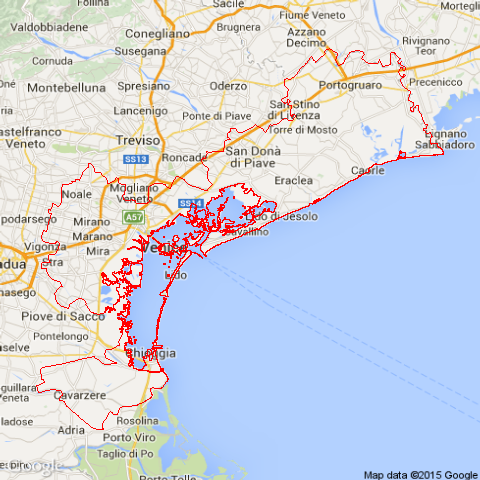
\includegraphics[width=0.46\textwidth]{Immagini/Ven_poligoni.png}   
   }
	\subfigure[Poligoni scelti]
   {
   \label{fig:Ven_poligoniscelti}
	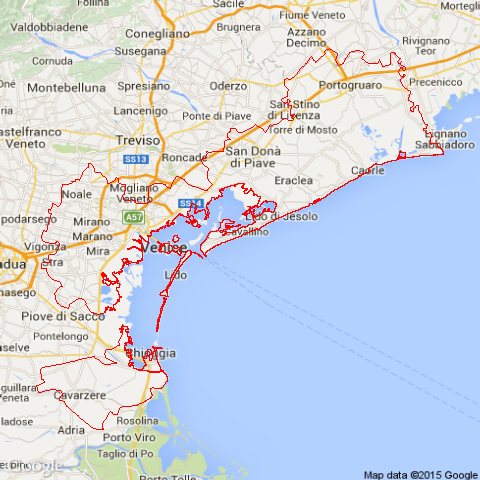
\includegraphics[width=0.46\textwidth]{Immagini/Ven_poligoniscelti.png}
   }
	\caption{Poligoni disponibili nel pacchetto \textit{raster}}
	\label{fig:Ven_poligoni}
\end{figure}

Oltre all'entroterra (composto da due poligoni) stati scelte solo le più più rilevanti isole della laguna a livello di popolazione e turismo: Venezia, Murano, Lido di Venezia, Pellestrina e Chioggia (composta da due poligoni). In fig. \ref{fig:Ven_poligoni} sono visualizzati i poligoni disponibili e quelli scelti per l'analisi. Come sarà indicato nel paragrafo successivo, tutte queste isole sono state trattate per la riduzione dei vertici e, per creare un poligono unico, sono state unite tra loro con ponti dove era possibile. Tra le isole collegate solamente via mare con il resto del territorio sono stati simulati ponti in corrispondenza delle trafficate linee di trasporto pubblico con traghetto. 

\subsection{Regression splines}

Per ridurre l'elevato numero di vertici di ognuno dei poligoni considerati si è scelto di ricorrere ad un'analisi di smoothing di dati funzionali. Ad ogni poligono è associata una coppia di funzioni: la latitudine e la longitudine rispetto all'ascissa curvilinea (disponibili per punti, corrispondenti ai vertici) che sono state rappresentate in basi e valutate in un mumero molto inferiore di punti, con i quali si è costruita la nuova definizione della regione.

Per avere una rappresentazione tramite funzioni di base di queste funzioni sono state provate più tecniche e la scelta definitiva è ricaduta sulle \textit{Regression Splines} cubiche senza penalizzazione della derivata seconda. Infatti i risultati non sono stati migliori negli altri casi a causa della zona interna alla laguna di Venezia, fortemente frastagliata: ad esempio penalizzare la derivata seconda eliminava troppe asperità presenti sulle coste del territorio, mentre con \textit{Kernel Smoothing} sono state ricavate regioni che, dopo la triangolazione, presentavano troppi triangoli composti solamente da punti di frontiera (e quindi senza dati) rispetto agli altri metodi.

Una volta fissato un ragionevole numero di punti con cui descrivere la regione sono stati eseguiti più tentativi per decidere il miglior numero di basi necessario per descrivere le due funzioni. Il criterio di scelta è stato complesso, poichè sono stati esclusi i valori che generavano intersezioni nella nuova descrizione della regione e comuni esterni alla frontiera. Ma la scelta del miglior numero di basi per \textit{Regression Splines} è ricaduta sul valore che, una volta eseguito lo smoothing della regione, causava la minor distanza tra i nuovi punti della regione e il poligono iniziale. In fig. \ref{fig:Ven_ent1} è riportato il risultato dello smoothing sul primo poligono, che descrive l'entroterra della provincia di Venezia (nella versione definitiva ha 100 punti, molti meno dei 10538 iniziali).  

\begin{figure}[t]
	\centering
	\begin{minipage}{.32\textwidth}
	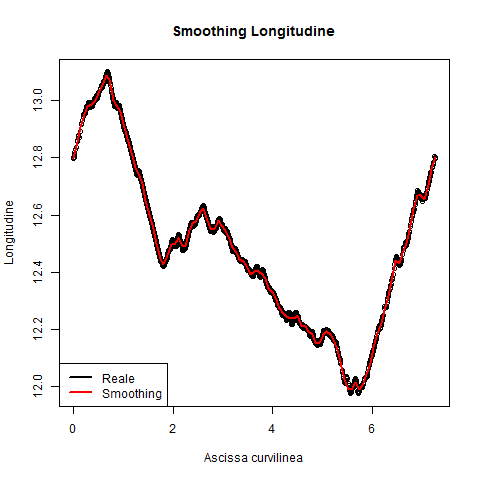
\includegraphics[width=\textwidth]{Immagini/Ven_Longitudine.png}
	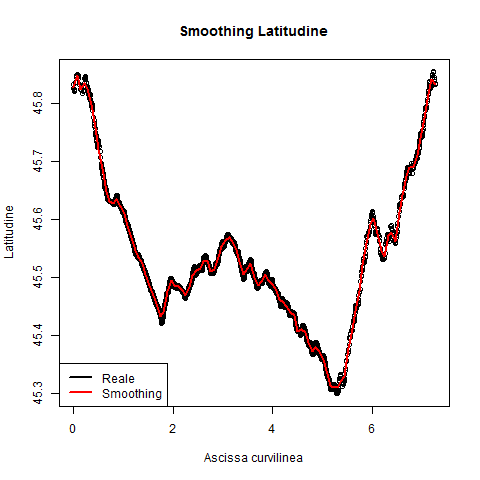
\includegraphics[width=\textwidth]{Immagini/Ven_Latitudine.png}
	\end{minipage}%
	\begin{minipage}{.64\textwidth}
	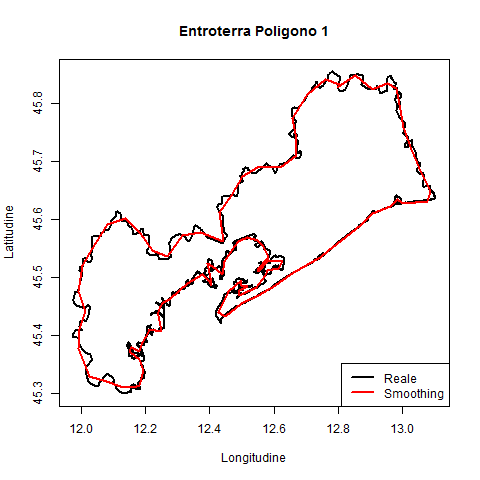
\includegraphics[width=\textwidth]{Immagini/Ven_Regione.png}
	\end{minipage}
	\caption{Smoothing con \textit{Regression Splines} cubiche per il primo poligono dell'entroterra della provincia di Venezia}
	\label{fig:Ven_ent1}
\end{figure}

Dopo aver ripetuto l'analisi per ognuna delle isole elencate precedentemente, la descrizione finale è stata ricavata unendo tra loro tutti i nuovi poligoni. In seguito è stata eliminata una zona costiera dell'entroterra della laguna di Venezia che, sebbene sia presente sia in \textit{raster} che nei grafici di Google Maps, corrisponde ad una parte fangosa e paludosa e quindi disabitata. Non essendo possibile che su di essa siano prodotti rifiuti è stata tagliata dalla regione. Per questo motivo si troverà sempre una zona non analizzata sui grafici con mappe da Google Maps. In fig. \ref{fig:Ven_rgm} è riportata la descrizione finale del dominio con i punti spaziali considerati (si consulti anche la sezione successiva).
\begin{figure}[t]
	\centering
	\subfigure[Provincia di Venezia]
   {
   \label{fig:Ven_rgm_tot}
	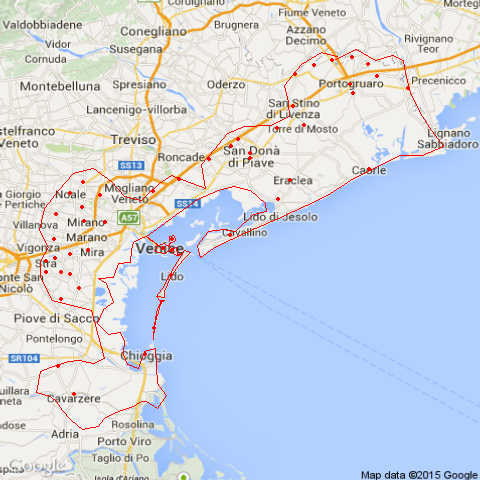
\includegraphics[width=0.46\textwidth]{Immagini/Ven_punti.png}   
   }
	\subfigure[Zoom della laguna]
   {
   \label{fig:Ven_rgm_zoom}
	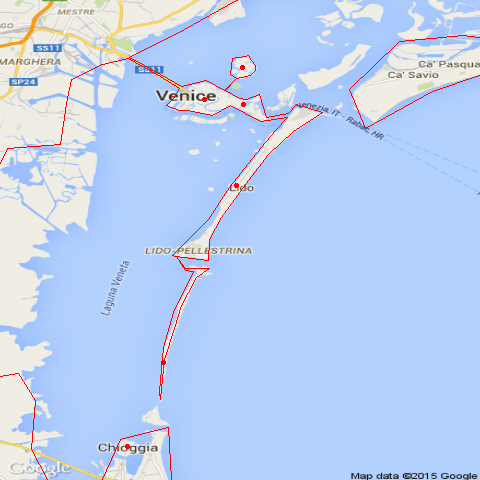
\includegraphics[width=0.46\textwidth]{Immagini/Ven_puntizoom.png}
   }
	\caption{Frontiera e punti spaziali per la provincia di Venezia}
	\label{fig:Ven_rgm}
\end{figure}

\subsection{Scelte particolari tra i comuni}
\label{sez:comunireplicati}

L'uso di valori pro capite per rifiuti e posti letto consente di replicare il dato del comune anche su altri punti in cui risulta necessario. Ad esempio le isole di Murano, Lido di Venezia e Pellestrina non sono sedi di comune, ma si riferiscono a Venezia. Quindi il dato di Venezia è stato replicato in queste isole ad ogni anno, per avere un valore di riferimento in quanto zone distaccate. Come si può notare in fig. \ref{fig:Ven_rgm_zoom} anche nell'isola di Venezia è stato duplicato il dato, per avere una triangolazione  senza troppi triangoli composti solo da punti di frontiera in una zona di particolare rilevanza.

Un caso particolare riguarda il comune di Cavallino-Treporti, che è stato istituito nel 1999 con una parte dei territori del comune di Venezia. La separazione all'interno dei dati, però, è presente dal 2002. Di conseguenza prima di questo anno il dato in Cavallino-Treporti è una replica del dato di Venezia.

\subsection{Triangolazione del dominio}

La triangolazione è stata prodotta tramite il pacchetto R \textit{RTriangle}. Poichè nella zona ad est il numero di capoluoghi di comune (e quindi di nodi della triangolazione) è minore rispetto al resto della regione, è stata fissata un'area massima per i triangoli generati da \textit{RTriangle}. Questo ha reso la triangolazione più fitta anche dove non lo sarebbe stata, e garantirà una stima della risposta più precisa nella zona balneare che, come si potrà notare in seguito, ha una grande importanza per la distribuzione dei rifiuti. Affinchè questo sia possibile sono stati aggiuhnti nuovi punti spaziali, che restano senza dato per tutta l'analisi. In fig. \ref{fig:Ven_triang} si ha la triangolazione finale che sarà usata da ora in avanti.

\begin{figure}[t]
\centering
\subfigure[Provincia di Venezia]
   {
   \label{fig:Ven_triang_tot}
	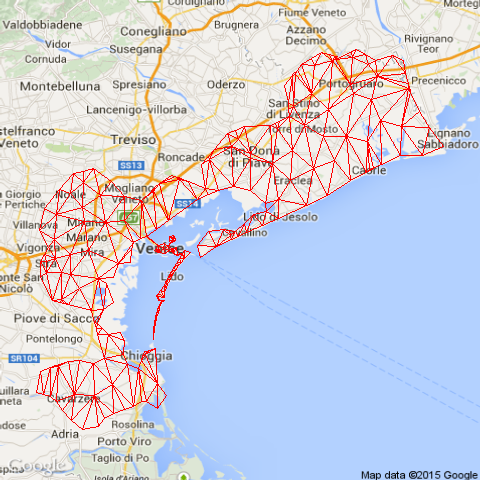
\includegraphics[width=0.46\textwidth]{Immagini/Ven_triang.png}   
   }
\subfigure[Zoom della laguna]
   {
   \label{fig:Ven_triang_zoom}
	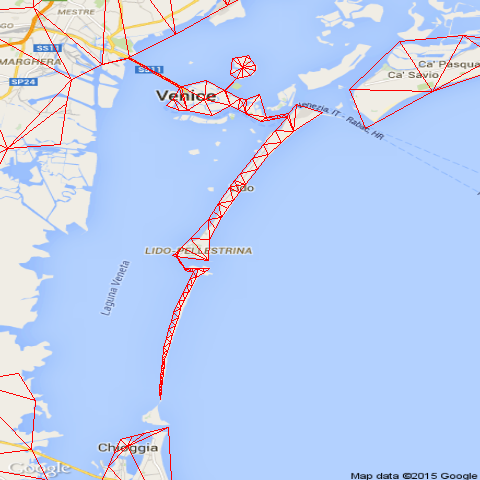
\includegraphics[width=0.46\textwidth]{Immagini/Ven_triangzoom.png}
   }
\caption{Triangolazione della provincia di Venezia}
\label{fig:Ven_triang}
\end{figure}

In conclusione, il dominio è descritto da 414 punti (41 con dati, 373 di frontiera o aggiunti dalla triangolazione) e da 475 triangoli.

\section{Analisi preliminare dei dati}
Prima di eseguire l'analisi, è opportuno avere una visualizzazione dei dati sul dominio della provincia di Venezia. In fig. \ref{fig:Ven_bubbledati} sono riportati i bubbleplot dei dati, che permettono di avere un'idea del fenomeno in spazio e tempo.
\newpage
\begin{figure}[H]
	\centering
	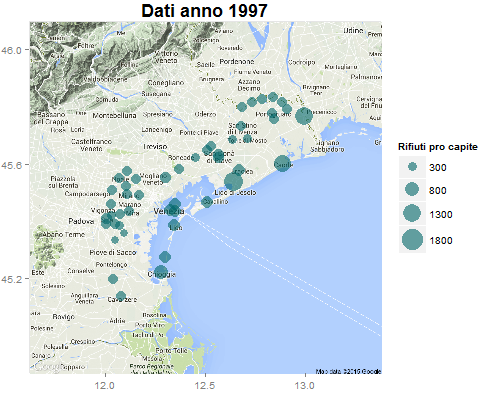
\includegraphics[trim=0cm 0cm 0cm 0cm,clip=true,width=0.45\textwidth]{Immagini/venezia_dati/Dati1997.png}
	%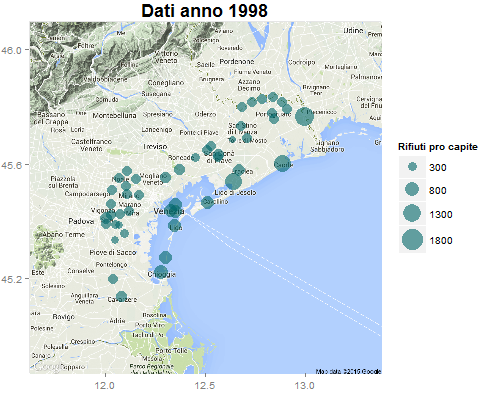
\includegraphics[trim=0cm 0cm 0cm 2cm,clip=true,width=0.45\textwidth]{Immagini/venezia_dati/Dati1998.png}
	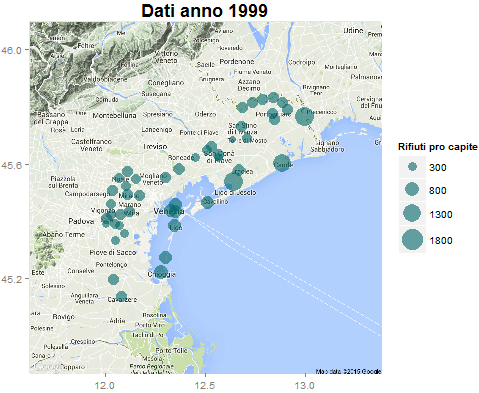
\includegraphics[trim=0cm 0cm 0cm 0cm,clip=true,width=0.45\textwidth]{Immagini/venezia_dati/Dati1999.png}
	%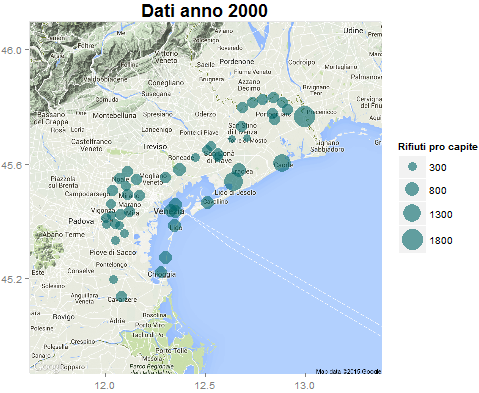
\includegraphics[trim=0cm 0cm 0cm 2cm,clip=true,width=0.45\textwidth]{Immagini/venezia_dati/Dati2000.png}
	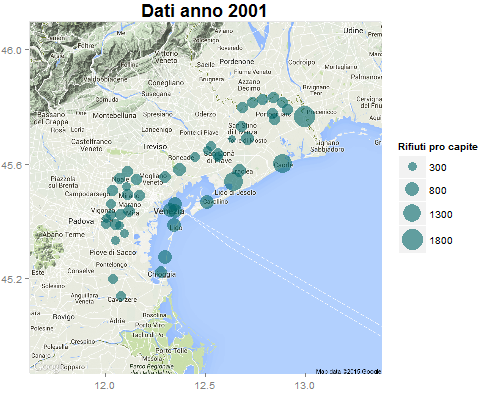
\includegraphics[trim=0cm 0cm 0cm 0cm,clip=true,width=0.45\textwidth]{Immagini/venezia_dati/Dati2001.png}
	%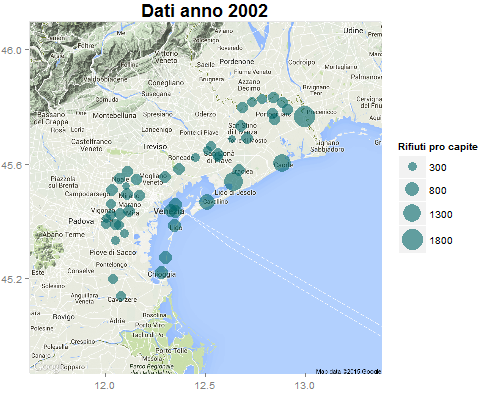
\includegraphics[trim=0cm 0cm 0cm 2cm,clip=true,width=0.45\textwidth]{Immagini/venezia_dati/Dati2002.png}
	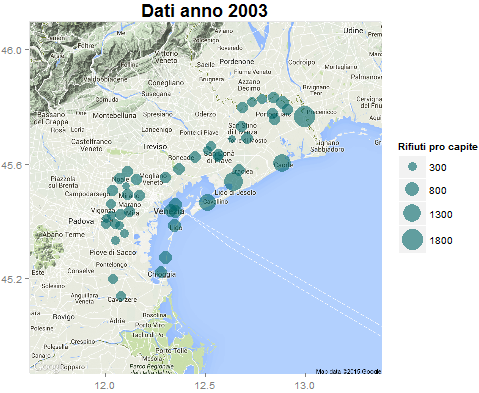
\includegraphics[trim=0cm 0cm 0cm 0cm,clip=true,width=0.45\textwidth]{Immagini/venezia_dati/Dati2003.png}
	%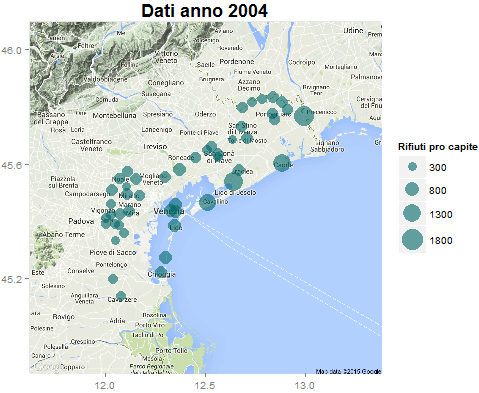
\includegraphics[trim=0cm 0cm 0cm 2cm,clip=true,width=0.45\textwidth]{Immagini/venezia_dati/Dati2004.png}
	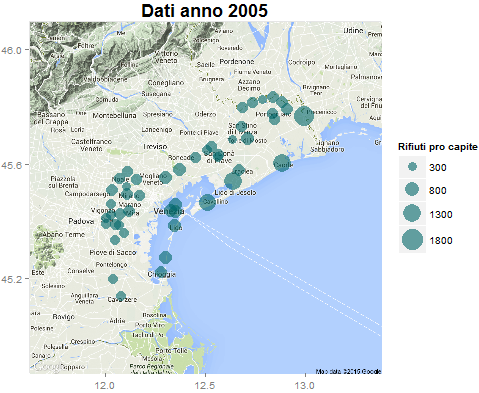
\includegraphics[trim=0cm 0cm 0cm 0cm,clip=true,width=0.45\textwidth]{Immagini/venezia_dati/Dati2005.png}
	%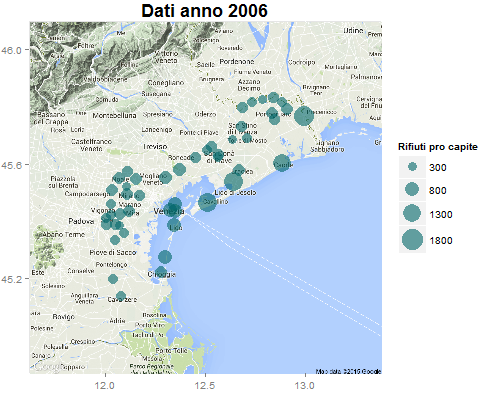
\includegraphics[trim=0cm 0cm 0cm 2cm,clip=true,width=0.45\textwidth]{Immagini/venezia_dati/Dati2006.png}
	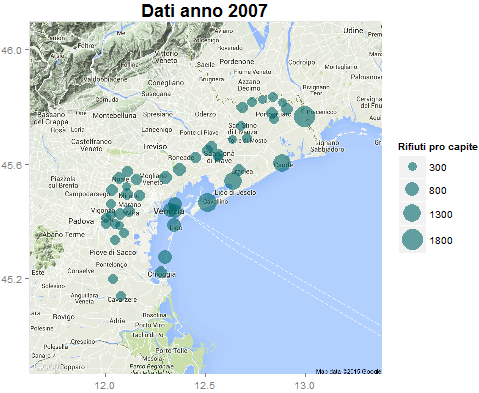
\includegraphics[trim=0cm 0cm 0cm 0cm,clip=true,width=0.45\textwidth]{Immagini/venezia_dati/Dati2007.png}
	%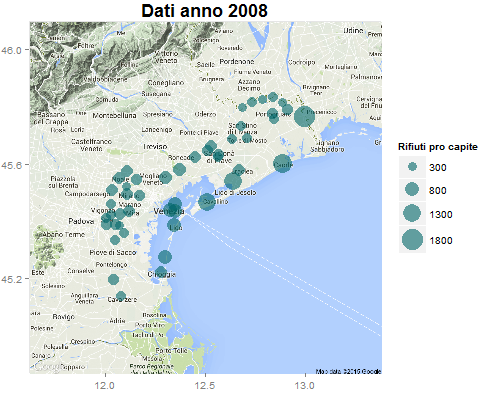
\includegraphics[trim=0cm 0cm 0cm 2cm,clip=true,width=0.45\textwidth]{Immagini/venezia_dati/Dati2008.png}
	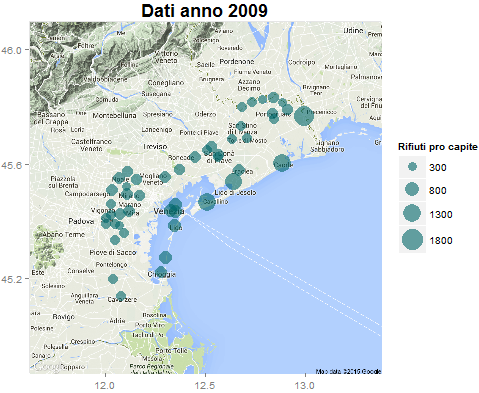
\includegraphics[trim=0cm 0cm 0cm 0cm,clip=true,width=0.45\textwidth]{Immagini/venezia_dati/Dati2009.png}
	%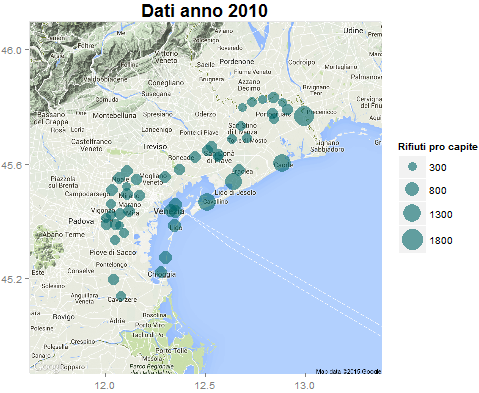
\includegraphics[trim=0cm 0cm 0cm 2cm,clip=true,width=0.45\textwidth]{Immagini/venezia_dati/Dati2010.png}
	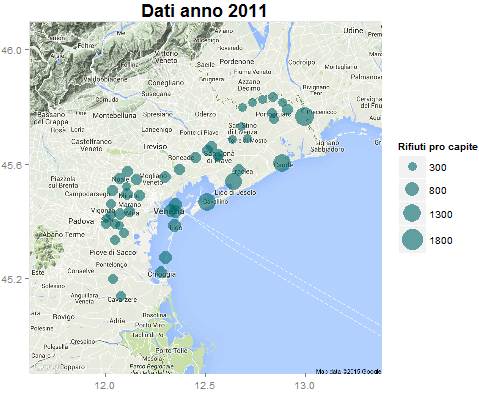
\includegraphics[trim=0cm 0cm 0cm 0cm,clip=true,width=0.45\textwidth]{Immagini/venezia_dati/Dati2011.png}
	\caption{Bubbleplot delle misurazioni della produzione di rifiuti urbani pro capite ogni due anni dal 1997 al 2011.}
	\label{fig:Ven_bubbledati}
\end{figure}
\newpage
\begin{figure}[H]
	\centering
	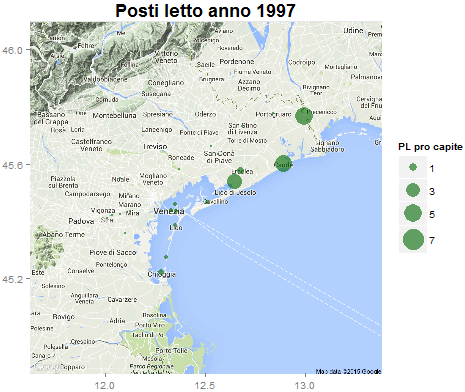
\includegraphics[trim=0cm 0cm 0cm 0cm,clip=true,width=0.45\textwidth]{Immagini/venezia_dati/PL1997.png}
	%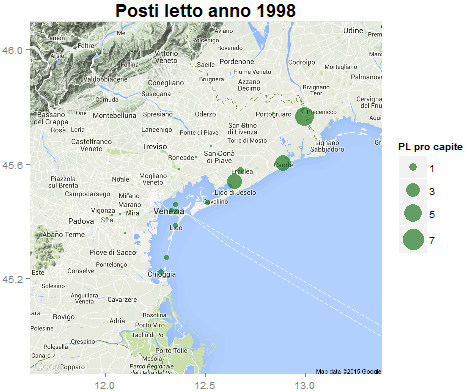
\includegraphics[trim=0cm 0cm 0cm 2cm,clip=true,width=0.45\textwidth]{Immagini/venezia_dati/PL1998.png}
	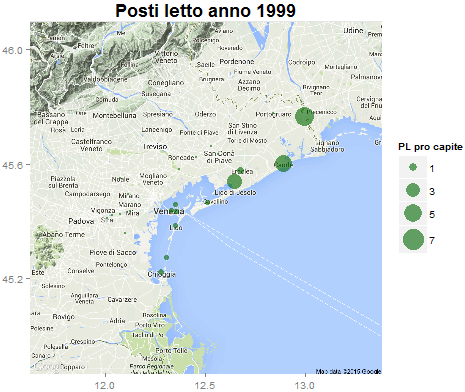
\includegraphics[trim=0cm 0cm 0cm 0cm,clip=true,width=0.45\textwidth]{Immagini/venezia_dati/PL1999.png}
	%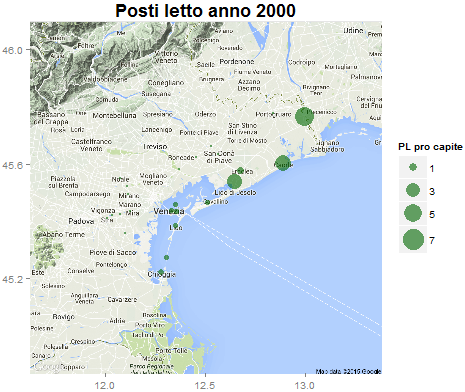
\includegraphics[trim=0cm 0cm 0cm 2cm,clip=true,width=0.45\textwidth]{Immagini/venezia_dati/PL2000.png}
	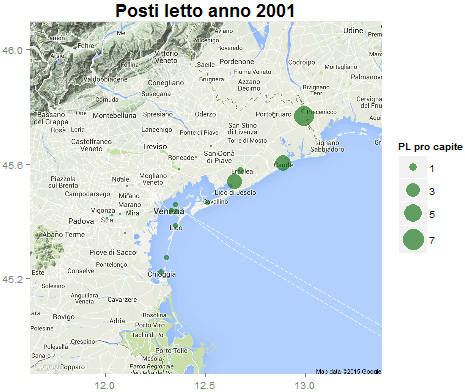
\includegraphics[trim=0cm 0cm 0cm 0cm,clip=true,width=0.45\textwidth]{Immagini/venezia_dati/PL2001.png}
	%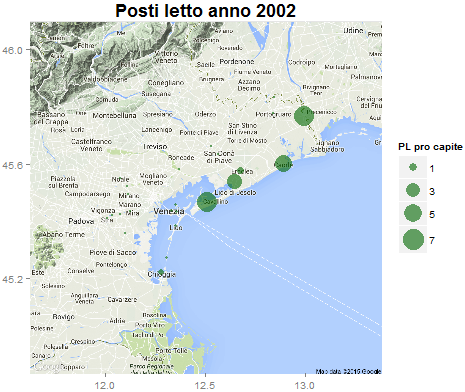
\includegraphics[trim=0cm 0cm 0cm 2cm,clip=true,width=0.45\textwidth]{Immagini/venezia_dati/PL2002.png}
	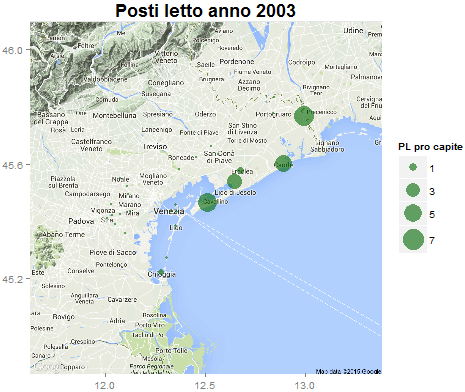
\includegraphics[trim=0cm 0cm 0cm 0cm,clip=true,width=0.45\textwidth]{Immagini/venezia_dati/PL2003.png}
	%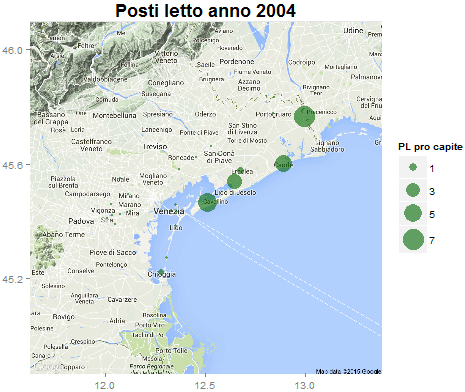
\includegraphics[trim=0cm 0cm 0cm 2cm,clip=true,width=0.45\textwidth]{Immagini/venezia_dati/PL2004.png}
	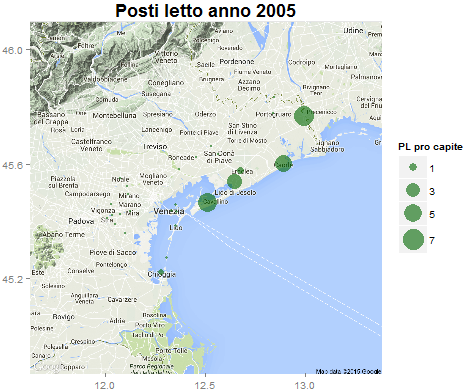
\includegraphics[trim=0cm 0cm 0cm 0cm,clip=true,width=0.45\textwidth]{Immagini/venezia_dati/PL2005.png}
	%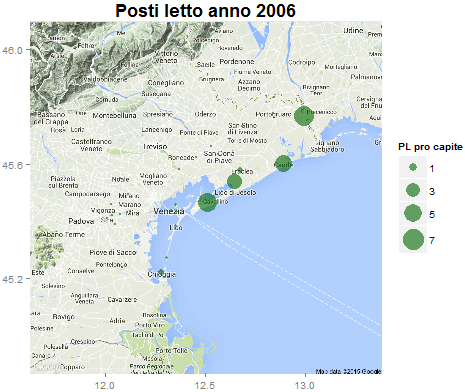
\includegraphics[trim=0cm 0cm 0cm 2cm,clip=true,width=0.45\textwidth]{Immagini/venezia_dati/PL2006.png}
	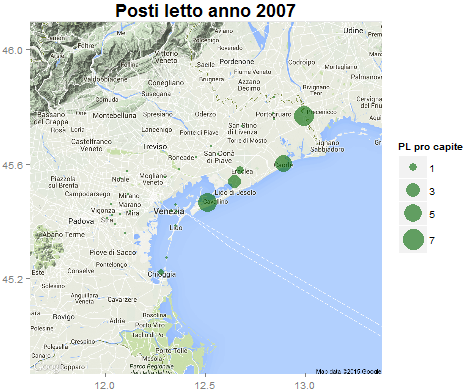
\includegraphics[trim=0cm 0cm 0cm 0cm,clip=true,width=0.45\textwidth]{Immagini/venezia_dati/PL2007.png}
	%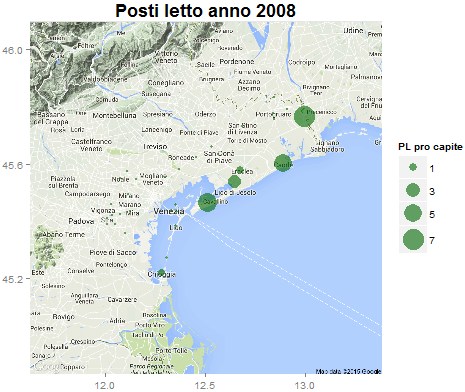
\includegraphics[trim=0cm 0cm 0cm 2cm,clip=true,width=0.45\textwidth]{Immagini/venezia_dati/PL2008.png}
	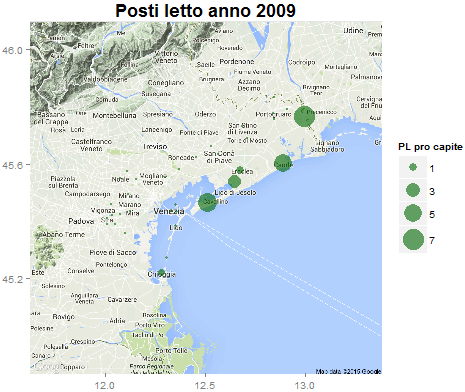
\includegraphics[trim=0cm 0cm 0cm 0cm,clip=true,width=0.45\textwidth]{Immagini/venezia_dati/PL2009.png}
	%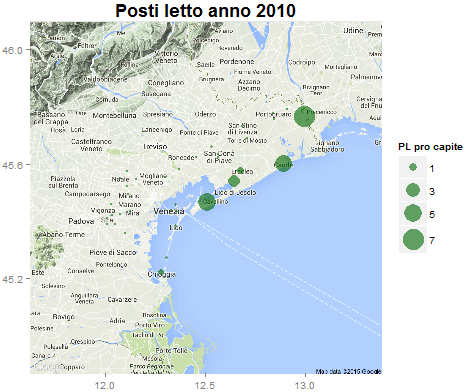
\includegraphics[trim=0cm 0cm 0cm 2cm,clip=true,width=0.45\textwidth]{Immagini/venezia_dati/PL2010.png}
	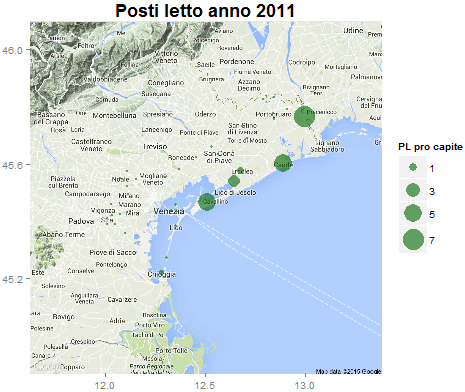
\includegraphics[trim=0cm 0cm 0cm 0cm,clip=true,width=0.45\textwidth]{Immagini/venezia_dati/PL2011.png}
	\caption{Bubbleplot dei posti letto pro capite ogni due anni dal 1997 al 2011.}
	\label{fig:Ven_bubblePL}
\end{figure}
\newpage
Da questa analisi iniziale si può ipotizzare che il modello mostri una produzione di rifiuti più alta nella zona balneare della regione e che non abbia grosse variazioni nel tempo, poichè i dati sono più o meno simili negli anni. 

Gli stessi grafici sono stati ripetuti in fig. \ref{fig:Ven_bubblePL} per il numero di posti letto pro capite. In questo caso, però, si può evidenziare un andamento diverso. Si può notare che il numero di posti letto assume valori maggiori nella zona balneare rispetto al resto della regione. Contrariamente a quello che ci si aspettava, non si hanno molto posti letto nell'isola di Venezia. Invece si ha una grossa variazione nel comune di Cavallino-Treporti dopo la separazione dal comune di Venezia (si nota che il raggio della bolla aumenta notevolmente dopo il 2002). Questo indica che i posti letto sono in realtà numerosi in Cavallino-Treporti, ma quando era unito al comune di Venezia questo effetto non poteva essere notato in modo così dettagliato. Ci si può quindi aspettare che la funzione stimata presenti un comportamento differente in Cavallino-Treporti nelle due situazioni.


\section{Applicazione del modello senza covariata}

\subsection{Ricerca del miglior $\underline \lambda$}
Le basi in spazio scelte per l'applicazione del modello in questo caso sono gli elementi finiti lineari. Ad ognuno dei punti spaziali (interni o di frontiera) è associata una funzione di base, coerentemente con la triangolazione prodotta. Di conseguenza si ha $N=414$ mentre il numero di punti con dati $n$ è minore ed è pari a 41.

In tempo, esattamente come nel caso del dominio a forma di C, sono state scelte come funzioni di base le B-splines cubiche. L'intervallo temporale per la descrizione del dominio è $[1997,2011]$ e i dati sono disponibili con cadenza annuale. Anche in questo caso si assume che il numero di basi sia pari al numero di istanti temporali a disposizione, quindi $M=m=15$.

Prima di calcolare i risultati dell'analisi occorre fissare i parametri $\lambda_S$ e $\lambda_T$. Il procedimento è perfettamente analogo a quello ricavato nel caso del dominio a forma di C, minimizzando la quantità $GCV(\underline \lambda)$ in (CITAZIONE NECESSARIA). In tab. \ref{tab:Ven} sono disponibili i risultati.

\newpage
\begin{table}[h]
\renewcommand{\arraystretch}{1.3}
\setlength{\tabcolsep}{2mm}
\centering
	\begin{tabular}{!{\vrule width 1.2pt}c!{\vrule width 1.2pt}c!{\vrule width 1.2pt}}
	\noalign{\hrule height 1.2pt}
	Intervalli per $\log_{10}\lambda_S$ e $\log_{10}\lambda_T$& Miglior valore											\\
	\noalign{\hrule height 1.2pt}
	$\log_{10}\lambda_S \in \{-12,-11,\ldots,+1\}$ 	& \multirow{2}{*}{$\underline \lambda = (10^{-10},10^{0})$} 			\\
	\cline{1-1}
	$\log_{10}\lambda_T \in \{-8,-7,\ldots,+1\}$		& 															\\	
	\noalign{\hrule height 1.2pt}
	$\log_{10}\lambda_S \in \{-11,-10.5,\ldots,-9\}$ 	& \multirow{2}{*}{$\underline \lambda = (10^{-9.5},10^{0})$} 		\\
	\cline{1-1}
	$\log_{10}\lambda_T \in \{-1,-0.5,\ldots,+1\}$	& 															\\	
	\noalign{\hrule height 1.2pt}
	$\log_{10}\lambda_S \in \{-10,-9.875,\ldots,-9\}$ 	& \multirow{2}{*}{$\underline \lambda = (10^{-9.625}, 10^{0})$}	\\
	\cline{1-1}
	$\log_{10}\lambda_T \in \{-0.5,-0.375,\ldots,+0.5\}$		& 			\\	
	\noalign{\hrule height 1.2pt}
	\end{tabular}
\caption{Analisi di $\mathrm{GCV}(\protect\underline{\lambda})$ per la provincia di Venezia, caso senza covariata}
\label{tab:Ven}
\end{table}

\subsection{Risultati}
La produzione dei rifiuti è stata analizzata con $\underline \lambda = (10^{-9.625}, 10^{0})$. In fig. \ref{fig:Ven_ris} sono riportati i risultati ottenuti nei 15 anni a disposizione. Questi grafici (grazie anche alla visualizzazione sulle mappe di Google Maps) permettono di studiare il profilo della funzione nei vari istanti temporali e di avere un'idea dell'evoluzione della produzione di rifiuti a livello geografico.
\newpage
\begin{figure}[H]
\centering
	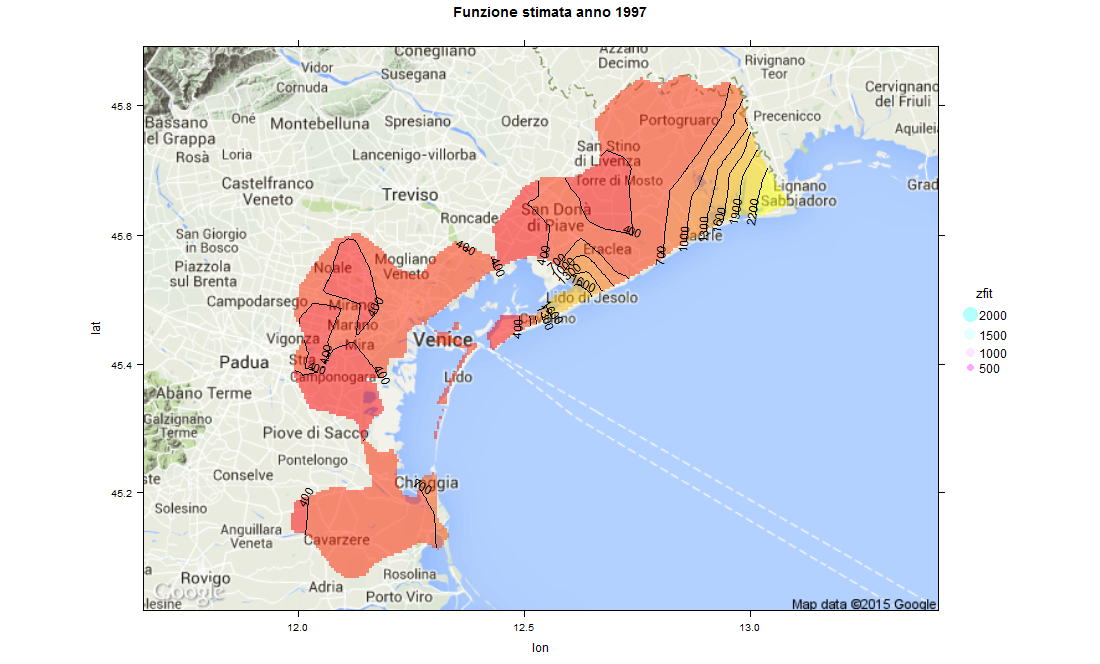
\includegraphics[trim=0cm 0cm 4cm 0cm,clip=true,width=0.32\textwidth]{Immagini/venezia_senza_covariate/Maps1997.png}
	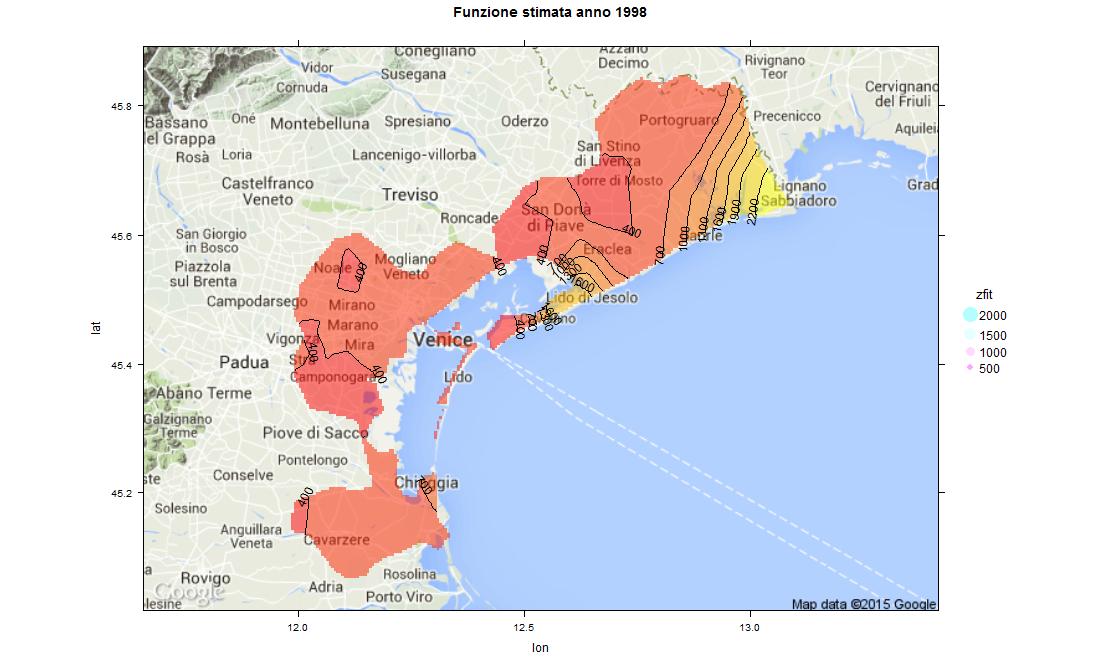
\includegraphics[trim=0cm 0cm 4cm 0cm,clip=true,width=0.32\textwidth]{Immagini/venezia_senza_covariate/Maps1998.png}
	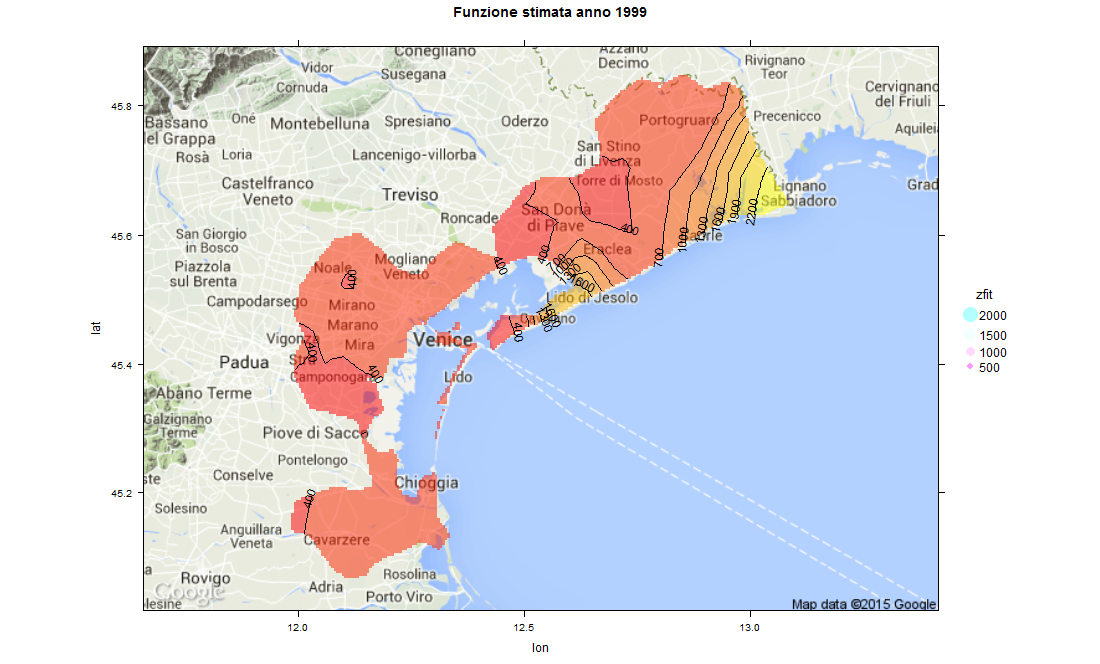
\includegraphics[trim=0cm 0cm 4cm 0cm,clip=true,width=0.32\textwidth]{Immagini/venezia_senza_covariate/Maps1999.png}
	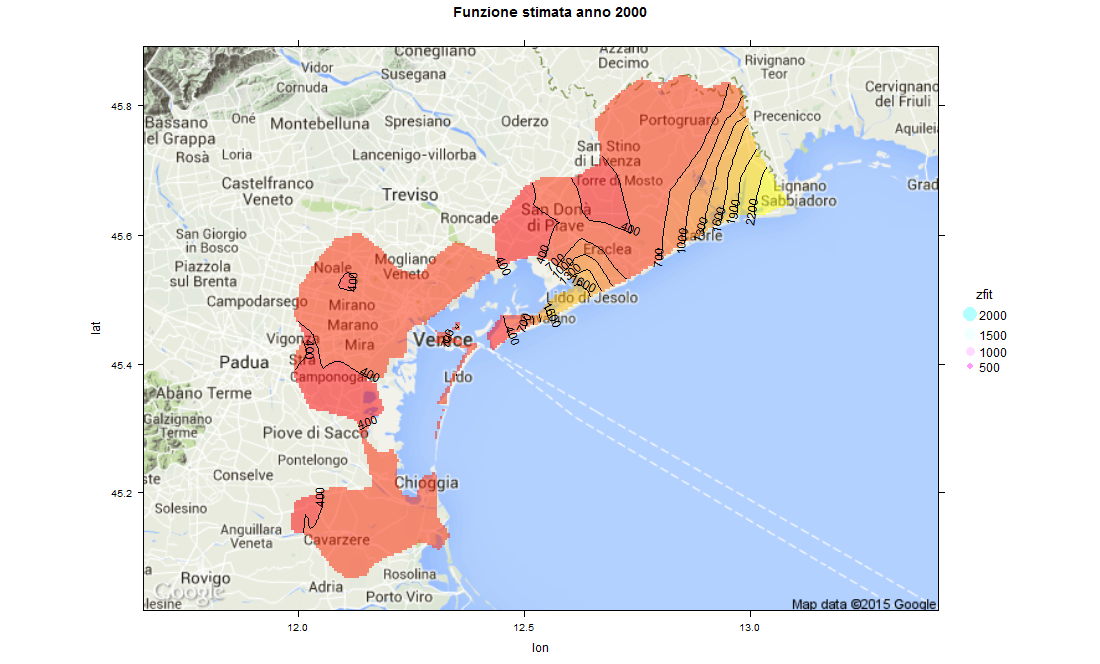
\includegraphics[trim=0cm 0cm 4cm 0cm,clip=true,width=0.32\textwidth]{Immagini/venezia_senza_covariate/Maps2000.png}
	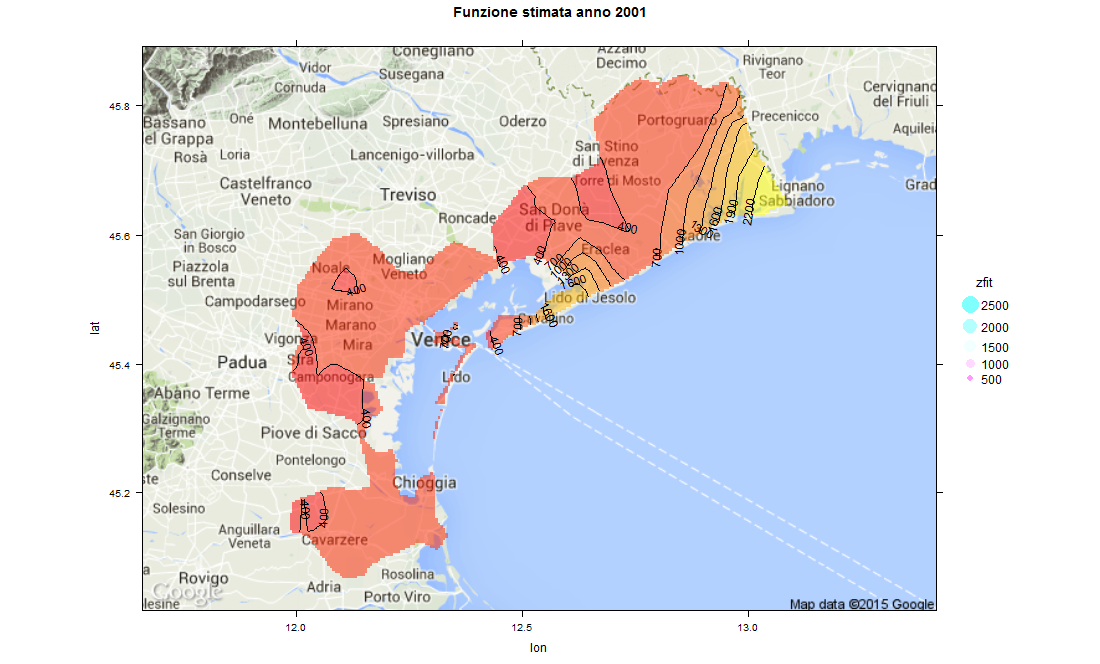
\includegraphics[trim=0cm 0cm 4cm 0cm,clip=true,width=0.32\textwidth]{Immagini/venezia_senza_covariate/Maps2001.png}
	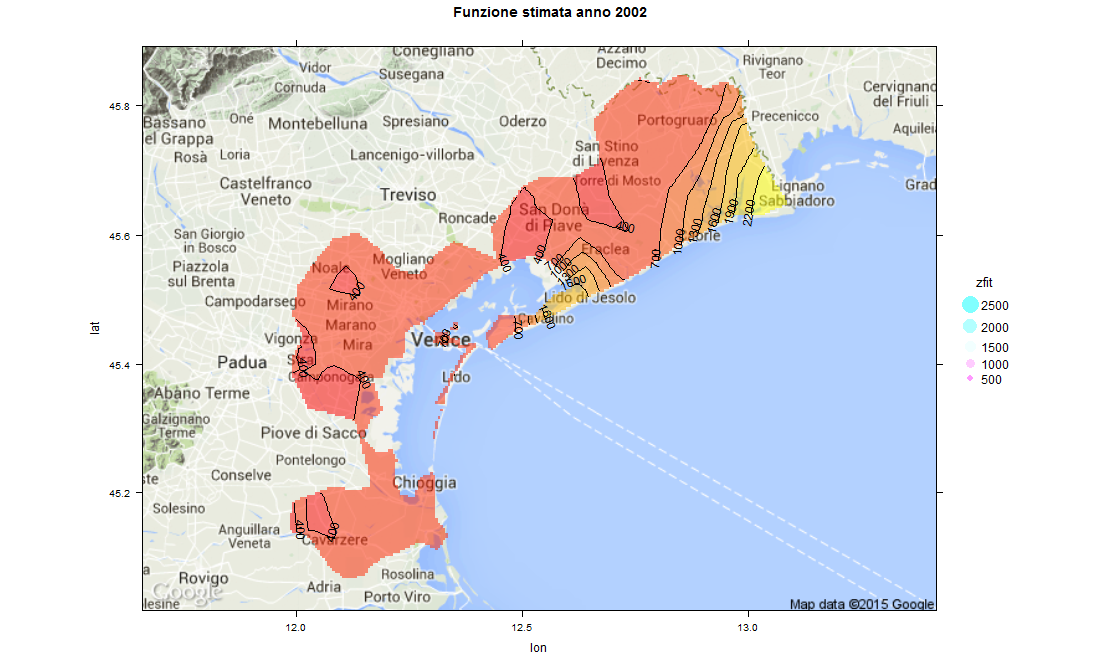
\includegraphics[trim=0cm 0cm 4cm 0cm,clip=true,width=0.32\textwidth]{Immagini/venezia_senza_covariate/Maps2002.png}
	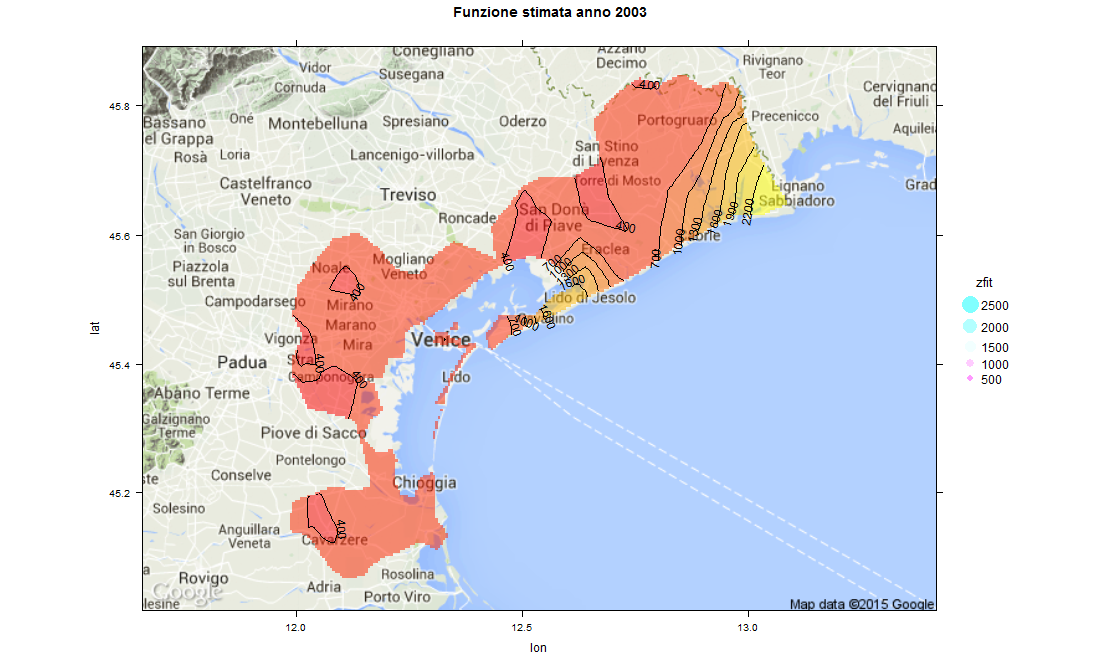
\includegraphics[trim=0cm 0cm 4cm 0cm,clip=true,width=0.32\textwidth]{Immagini/venezia_senza_covariate/Maps2003.png}
	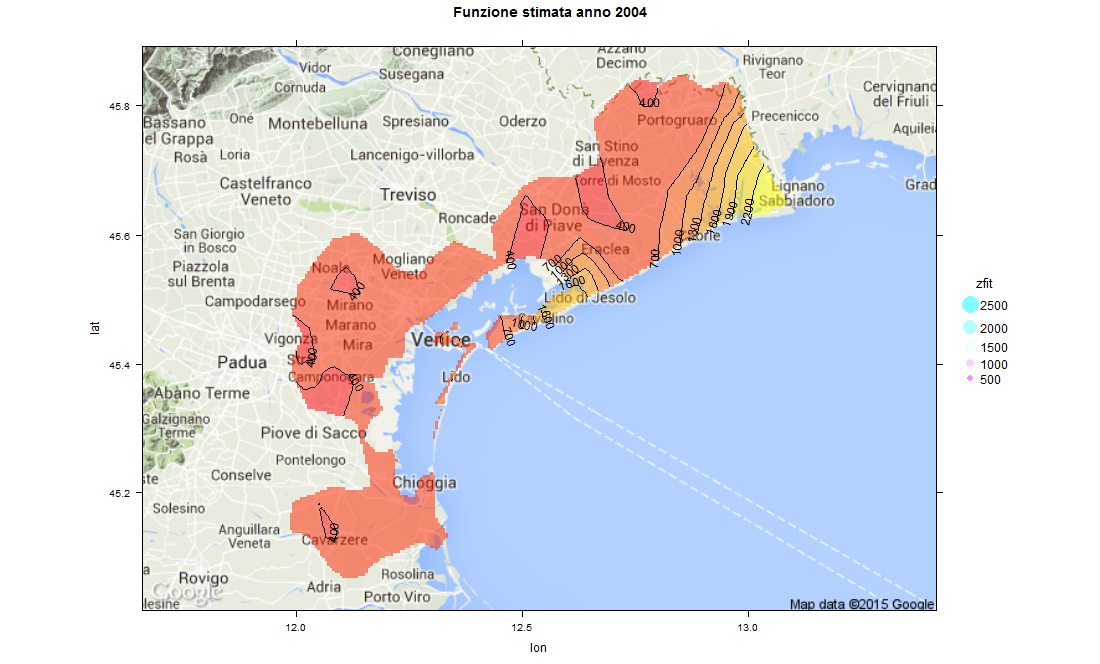
\includegraphics[trim=0cm 0cm 4cm 0cm,clip=true,width=0.32\textwidth]{Immagini/venezia_senza_covariate/Maps2004.png}
	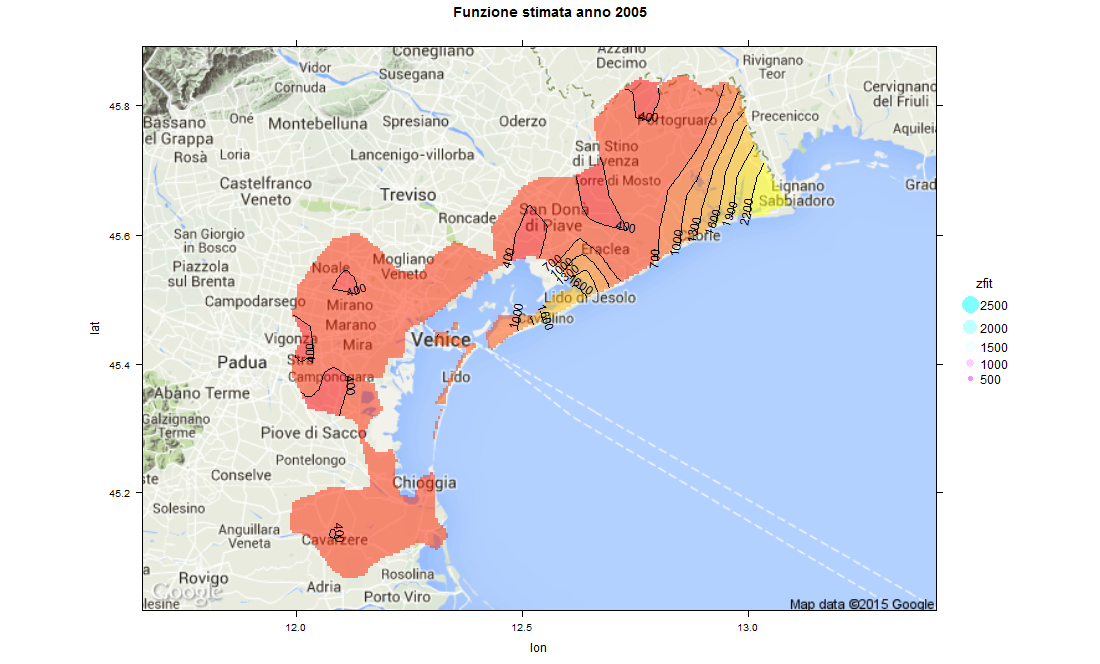
\includegraphics[trim=0cm 0cm 4cm 0cm,clip=true,width=0.32\textwidth]{Immagini/venezia_senza_covariate/Maps2005.png}
	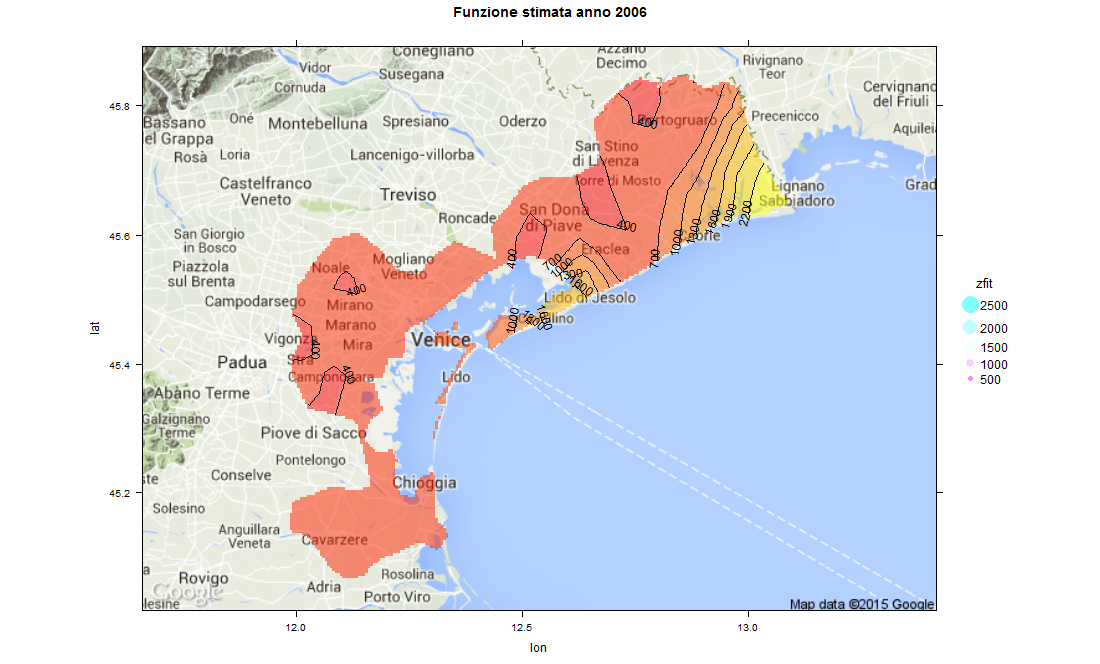
\includegraphics[trim=0cm 0cm 4cm 0cm,clip=true,width=0.32\textwidth]{Immagini/venezia_senza_covariate/Maps2006.png}
	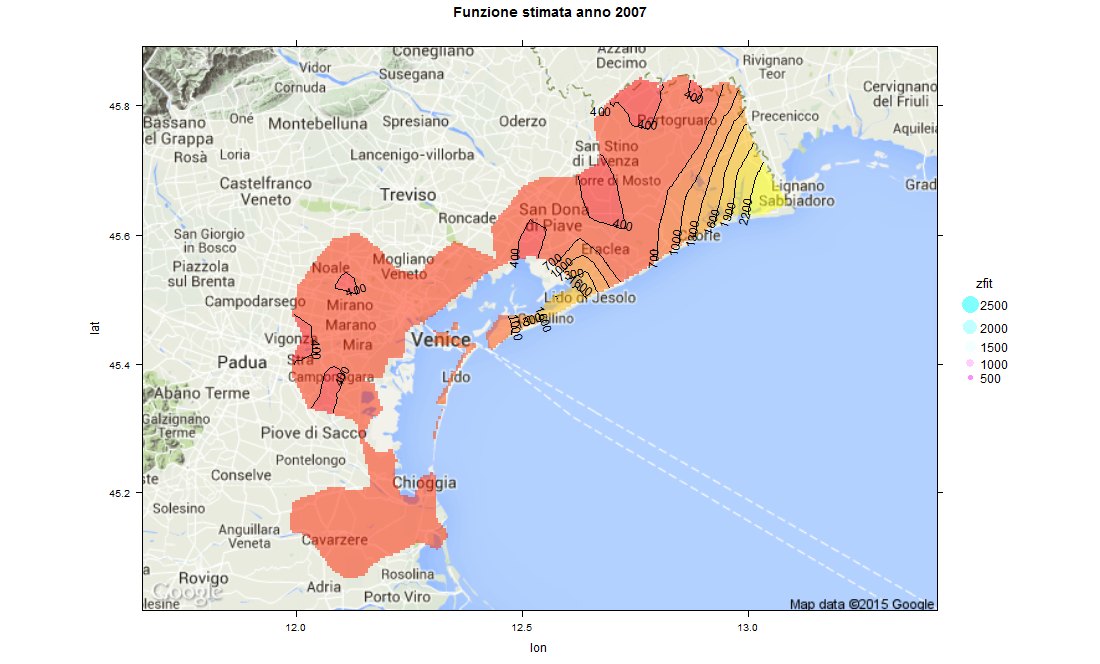
\includegraphics[trim=0cm 0cm 4cm 0cm,clip=true,width=0.32\textwidth]{Immagini/venezia_senza_covariate/Maps2007.png}
	\includegraphics[trim=0cm 0cm 4cm 0cm,clip=true,width=0.32\textwidth]{Immagini/venezia_senza_covariate/Maps2008.png}
	\includegraphics[trim=0cm 0cm 4cm 0cm,clip=true,width=0.32\textwidth]{Immagini/venezia_senza_covariate/Maps2009.png}
	\includegraphics[trim=0cm 0cm 4cm 0cm,clip=true,width=0.32\textwidth]{Immagini/venezia_senza_covariate/Maps2010.png}
	\includegraphics[trim=0cm 0cm 4cm 0cm,clip=true,width=0.32\textwidth]{Immagini/venezia_senza_covariate/Maps2011.png}
	\caption{Stima della funzione spazio-temporale della produzione dei rifiuti nella provincia di Venezia a tempi fissati dal 1997 al 2011, caso senza covariata.}
	\label{fig:Ven_ris}
\end{figure}
\newpage
Come si può notare dai grafici, ci sono due zone ad elevato valore di produzione dei rifiuti pro capite, corrispondenti a località con grande interesse turistico per le spiagge presenti. Ad est, tra le altre, si hanno le località turistiche di Bibione (confinante con Lignano Sabbiadoro, che però è oltre il confine) e Caorle. Scendendo verso sud-ovest si nota che anche Jesolo causa un innalzamento della funzione che descrive la risposta. La produzione dei rifiuti è particolarmente alta in queste zone turistiche e, contrariamente a ciò che si poteva immaginare, molto più di Venezia. Come già si notava dai bubbleplot in fig. \ref{fig:Ven_bubblePL}, il turismo sarà rilevante nell'analisi della produzione di rifiuti, e la causa non sarà Venezia (dove la produzione non è eccessivamente diversa dagli altri comuni) ma saranno le località balneari.

\begin{figure}[t]
	\centering
	\subfigure[Venezia]
   {
	\includegraphics[width=0.31\textwidth]{Immagini/venezia_senza_covariate/Venezia.png}   
   }
	\subfigure[Cavallino-Treporti]
   {
	\includegraphics[width=0.31\textwidth]{Immagini/venezia_senza_covariate/Cavallino-Treporti.png}
   }
	\subfigure[Chioggia]
   {
	\includegraphics[width=0.31\textwidth]{Immagini/venezia_senza_covariate/Chioggia.png}   
   }
	\subfigure[Jesolo]
   {
	\includegraphics[width=0.31\textwidth]{Immagini/venezia_senza_covariate/Jesolo.png}
   }
	\subfigure[Caorle]
   {
	\includegraphics[width=0.31\textwidth]{Immagini/venezia_senza_covariate/Caorle.png}   
   }
	\subfigure[S. Michele al Tagliamento]
   {
	\includegraphics[width=0.31\textwidth]{Immagini/venezia_senza_covariate/SanMichelealTagliamento.png}
   }
	\caption{Stima della produzione dei rifiuti pro capite in alcuni comuni, caso senza covariata.}
	\label{fig:Ven_tempo}
\end{figure}

In fig. \ref{fig:Ven_tempo} sono tracciati gli sviluppi temporali stimati in alcuni comuni. I punti rossi corrispondono al dato misurato. La funzione stimata spiega bene l'andamento tracciato dai dati iniziali senza cadere nell'eccessiva interpolazione. Infatti lo smoothing imposto dal modello tramite la penalizzazione della derivata seconda in tempo permette di non avere variazioni repentine. Ad esempio nei grafici di Venezia e Cavallino-Treporti il cambio di andamento dovuto alla separazione del comune dal 2002 non ha provocato bruschi cambiamenti alla funzione ma è stato comunque colto dal modello. In Chioggia e in Jesolo si ha un calo generale della produzione dei rifiuti, mentre in San Michele al Tagliamento (comune di appartenenza di Bibione) e Caorle si hanno valori alti, a conferma dei grafici in \ref{fig:Ven_ris}.

\subsection{Analisi dei residui}

\begin{figure}[t]
	\centering
	\subfigure[$z_{ij}$ vs $e_{ij}$]
	{
	\includegraphics[width=0.46\textwidth]{Immagini/venezia_senza_covariate/Scatterplot1.png}  
   }
	\subfigure[$\hat{z}_{ij}$ vs $e_{ij}$]
   {
	\includegraphics[width=0.46\textwidth]{Immagini/venezia_senza_covariate/Scatterplot2.png}
   }
	\caption{Scatterplot dei residui, caso senza covariata}
	\label{fig:Ven_residui}
\end{figure}
Contrariamente a quanto fatto in precedenza nel caso di dominio a forma di C, non si può prescindere dall'analisi dei residui per verificare l'ipotesi di omogeneità in varianza. Tramite gli scatterplot in fig. \ref{fig:Ven_residui} si può concludere che l'ipotesi è rispettata poichè i residui si dispongono come una nuvola uniformemente distribuita intorno allo zero.


\section{Applicazione del modello con covariata}

\subsection{Ricerca del miglior $\underline \lambda$}
Le basi in spazio e in tempo sono esattamente le stesse del caso precedente. Prima di eseguire l'analisi, come al solito, occorre cercare buoni valori per $\underline \lambda$. Dalla tab. \ref{tab:Vencovar} si possono seguire le iterazioni eseguite e il risultato finale.
\newpage
\begin{table}[h]
\renewcommand{\arraystretch}{1.3}
\setlength{\tabcolsep}{2mm}
\centering
	\begin{tabular}{!{\vrule width 1.2pt}c!{\vrule width 1.2pt}c!{\vrule width 1.2pt}}
	\noalign{\hrule height 1.2pt}
	Intervalli per $\log_{10}\lambda_S$ e $\log_{10}\lambda_T$& Miglior valore											\\
	\noalign{\hrule height 1.2pt}
	$\log_{10}\lambda_S \in \{-12,-11,\ldots,+1\}$ 	& \multirow{2}{*}{$\underline \lambda = (10^{-8},10^{0})$} 			\\
	\cline{1-1}
	$\log_{10}\lambda_T \in \{-8,-7,\ldots,+1\}$		& 															\\	
	\noalign{\hrule height 1.2pt}
	$\log_{10}\lambda_S \in \{-9,-8.5,\ldots,-7\}$ 	& \multirow{2}{*}{$\underline \lambda = (10^{-8},10^{0})$} 		\\
	\cline{1-1}
	$\log_{10}\lambda_T \in \{-1,-0.5,\ldots,+1\}$	& 															\\	
	\noalign{\hrule height 1.2pt}
	$\log_{10}\lambda_S \in \{-8.5,-8.375,\ldots,-7.5\}$ 	& \multirow{2}{*}{$\underline \lambda = (10^{-7.750}, 10^{-0.125})$}	\\
	\cline{1-1}
	$\log_{10}\lambda_T \in \{-0.5,-0.375,\ldots,+0.5\}$		& 			\\	
	\noalign{\hrule height 1.2pt}
	\end{tabular}
\caption{Analisi di $\mathrm{GCV}(\protect\underline{\lambda})$ per la provincia di Venezia, caso con covariata}
\label{tab:Vencovar}
\end{table}

\subsection{Risultati}
Le analisi sono state eseguite con $\underline \lambda = (10^{-7.750}, 10^{-0.125})$. Come si può notare dai grafici in fig. \ref{fig:Vencovar_ris}, dove è riportata la stima della funzione $f(\underline p,t)$ in tutti i punti senza l'aggiunta della parte spiegata dalla covariata, nelle zone dove la produzione di rifiuti è massima si hanno ora i valori più bassi.
\newpage
\begin{figure}[H]
\centering
\includegraphics[trim=0cm 0cm 4cm 0cm,clip=true,width=0.32\textwidth]{Immagini/venezia_con_covariate/Maps1997.png}
\includegraphics[trim=0cm 0cm 4cm 0cm,clip=true,width=0.32\textwidth]{Immagini/venezia_con_covariate/Maps1998.png}
\includegraphics[trim=0cm 0cm 4cm 0cm,clip=true,width=0.32\textwidth]{Immagini/venezia_con_covariate/Maps1999.png}
\includegraphics[trim=0cm 0cm 4cm 0cm,clip=true,width=0.32\textwidth]{Immagini/venezia_con_covariate/Maps2000.png}
\includegraphics[trim=0cm 0cm 4cm 0cm,clip=true,width=0.32\textwidth]{Immagini/venezia_con_covariate/Maps2001.png}
\includegraphics[trim=0cm 0cm 4cm 0cm,clip=true,width=0.32\textwidth]{Immagini/venezia_con_covariate/Maps2002.png}
\includegraphics[trim=0cm 0cm 4cm 0cm,clip=true,width=0.32\textwidth]{Immagini/venezia_con_covariate/Maps2003.png}
\includegraphics[trim=0cm 0cm 4cm 0cm,clip=true,width=0.32\textwidth]{Immagini/venezia_con_covariate/Maps2004.png}
\includegraphics[trim=0cm 0cm 4cm 0cm,clip=true,width=0.32\textwidth]{Immagini/venezia_con_covariate/Maps2005.png}
\includegraphics[trim=0cm 0cm 4cm 0cm,clip=true,width=0.32\textwidth]{Immagini/venezia_con_covariate/Maps2006.png}
\includegraphics[trim=0cm 0cm 4cm 0cm,clip=true,width=0.32\textwidth]{Immagini/venezia_con_covariate/Maps2007.png}
\includegraphics[trim=0cm 0cm 4cm 0cm,clip=true,width=0.32\textwidth]{Immagini/venezia_con_covariate/Maps2008.png}
\includegraphics[trim=0cm 0cm 4cm 0cm,clip=true,width=0.32\textwidth]{Immagini/venezia_con_covariate/Maps2009.png}
\includegraphics[trim=0cm 0cm 4cm 0cm,clip=true,width=0.32\textwidth]{Immagini/venezia_con_covariate/Maps2010.png}
\includegraphics[trim=0cm 0cm 4cm 0cm,clip=true,width=0.32\textwidth]{Immagini/venezia_con_covariate/Maps2011.png}
\caption{Stima della funzione spazio-temporale della produzione dei rifiuti nella provincia di Venezia a tempi fissati dal 1997 al 2011, con covariata.}
\label{fig:Vencovar_ris}
\end{figure}

\begin{figure}[t]
	\centering
	\subfigure[Venezia]
   {
	\includegraphics[width=0.31\textwidth]{Immagini/venezia_con_covariate/Venezia.png}   
   }
	\subfigure[Cavallino-Treporti]
   {
	\includegraphics[width=0.31\textwidth]{Immagini/venezia_con_covariate/Cavallino-Treporti.png}
   }
	\subfigure[Chioggia]
   {
	\includegraphics[width=0.31\textwidth]{Immagini/venezia_con_covariate/Chioggia.png}   
   }
	\subfigure[Jesolo]
   {
	\includegraphics[width=0.31\textwidth]{Immagini/venezia_con_covariate/Jesolo.png}
   }
	\subfigure[Caorle]
   {
	\includegraphics[width=0.31\textwidth]{Immagini/venezia_con_covariate/Caorle.png}   
   }
	\subfigure[S. Michele al Tagliamento]
   {
	\includegraphics[width=0.31\textwidth]{Immagini/venezia_con_covariate/SanMichelealTagliamento.png}
   }
	\caption{Stima della parte funzionale della produzione dei rifiuti pro capite in alcuni comuni, con covariata.}
	\label{fig:Vencovar_tempo}
\end{figure}
\newpage
In fig. \ref{fig:Vencovar_tempo} si hanno anche i grafici della funzione stimata (senza il termine di covariata) in alcuni comuni. I punti tracciati in rosso rappresentano il dato, a cui è sottratta la covariata moltiplicata per $\hat{\beta}$ stimato. Non possono essere considerati come la parte di dati generati esattamente dalla funzione, ma come una loro buona approssimazione.

L'interpretazione del risultato in questo caso è legata all'alta affluenza turistica nelle zone balneari. Come si può notare dai grafici iniziali dalle fig. \ref{fig:Ven_bubbledati} e \ref{fig:Ven_bubblePL}, su tutta la zona costiera non si hanno solo i massimi dei rifiuti pro capite ma anche del numero di posti letto pro capite. Quindi non soltanto la produzione di rifiuti è massima nella zona balneare (come già si notava dalla funzione stimata nel caso senza covariata) ma anche l'attività turistica. In questo caso
$$
\hat{\beta}\approx284.05 \ .
$$
Più la covariata è alta, più è sottratta informazione alla funzione $f(\underline p,t)$, poichè $\hat{\beta}$ è costante in spazio e tempo. Perciò la funzione ha un profilo quasi simile ad una traslazione del caso senza covariate nel resto del dominio (in questa zona il numero di posti letto pro capite, come si nota in fig. \ref{fig:Ven_bubblePL}, è quasi costante) e ribassato nella zona balneare, a causa dell'alto contributo della covariata.

Interessante è quanto accade nel comune di Cavallino-Treporti, dove la funzione subisce una grossa variazione dopo la divisione dal comune di Venezia per l'aumento del numero dei posti letto. Attorno all'anno 2002 si ha uno stravolgimento dell'andamento della funzione. Tuttavia, essendo dovuto alla maggior precisione del dato in Cavallino-Treporti, è un cambiamento utile a spiegar meglio la risposta. Gli effetti dovuti alle propiretà di smoothing poste dal modello sono analoghi al caso senza covariata, si ha una spiegazione dell'andamento generale della funzione senza cogliere troppo il dato e senza interpolare. Nelle località dove si avevano i valori massimi nel caso senza covariata, ora si hanno i minimi a causa dei posti letto (in alcuni casi la funzione è addirittura negativa).

\subsection{Analisi dei residui}

\begin{figure}[t]
	\centering
	\subfigure[$z_{ij}$ vs $e_{ij}$]
	{
	\includegraphics[width=0.46\textwidth]{Immagini/venezia_con_covariate/Scatterplot2.png}  
	}
	\subfigure[$\hat{z}_{ij}$ vs $e_{ij}$]
   {
	\includegraphics[width=0.46\textwidth]{Immagini/venezia_con_covariate/Scatterplot3.png}
   }
	\caption{Scatterplot dei residui, caso con covariata}
	\label{fig:Vencovar_residui}
\end{figure}
Anche in questo caso è necessario controllare l'ipotesi di omoschedasticità dei residui. I risultati sono perfettamente analoghi al caso senza covariata e si può concludere che l'ipotesi è rispettata.
\newpage
\begin{figure}[h]
	\centering
	\includegraphics[width=0.45\textwidth]{Immagini/venezia_con_covariate/QQplot.png}   
   \caption{QQplot dei residui, caso con covariata}
	\label{fig:Ven_qqplot}
\end{figure}
Essendo presente una covariata, potrebbe essere interessante calcolare per essa intervalli di confidenza o verificare alcune ipotesi. Pertanto in questo caso è opportuno controllare anche l'eventuale gaussianità dei residui. Dal QQplot in fig. \ref{fig:Ven_qqplot}, troppo distante da una retta, e dal p-value del Shapiro-Wilk test, che è stimato minore di $2\times 10^{-16}$, si deduce che la gaussianità non può essere ipotizzata e quindi non è possibile calcolare intervalli di confidenza come fatto per il dominio a forma di C.


\end{document}